\chapter{Pilotná implementácia}
\label{kap:pilot} % id kapitoly pre prikaz ref

Za účelom rýchlejšieho testovania konceptov a poskytnutia lepšej predstavy o návrhoch opísaných v kapitole \ref{kap:prvy_navrh} vznikla pilotná implementácia vo forme webovej aplikácie obsahujúca všetky tri navrhované grafové reprezentácie. V jednotlivých podkapitolách je opísaná samotná realizácia tejto prvotnej verzie, ako aj zhodnotenie jej prínosu pre ďalšie iterácie.

\section{Používateľské rozhranie}
\label{sec:pilot_desc}

Ponúka štyri prednastavené dvojice jazyka logiky prvého rádu s jedným binárnym predikátom a štruktúrou pre tento jazyk. Každý z nich je zvolený tak, aby implementáciu demonštroval v rôznorodých scenároch. Interpretáciu binárneho predikátu je možné pomocou grafov aj upravovať, zmeny ostatných parametrov však nie sú podporované.

Na obrázku \ref{obr:demo_1} je zobrazená časť aplikácie predstavujúca práve zvolený jazyk a štruktúru. V ľavom hornom rohu sa nachádzajú jednotlivé prednastavené štruktúry, medzi ktorými môže užívateľ prepínať. Napravo od nich si zas užívateľ vyberá, ktoré grafové reprezentácie chce, aby sa mu naraz zobrazovali. Kontajner so štruktúrou, v spodnej častí obrázka,  obsahuje interpretácie konštánt, binárneho predikátu a všetkých unárnych predikátov. Je nutné podotknúť, že toto rozhranie slúži výhradne na efektívnejšiu demonštráciu grafových reprezentácií, nie je teda súčasťou samotného návrhu.

Časť aplikácie s grafmi je zachytená na obrázku \ref{obr:demo_2}. V tomto prípade sú zvolené pohľady na orientovaný a bipartitný graf. Je viditeľné, že táto implementácia ostala z veľkej časti verná návrhu. Orientovaný graf demonštruje panel so zvolenými unárnymi predikátmi, ktoré sa korektne zobrazujú v príslušných vrcholoch. V bipartitnom grafe je zas možné vrcholy reorganizovať, ale iba spôsobom špecifikovaným v návrhu \ref{sec:bipartite_graph_navrh}. Oba grafy podporujú vytváranie aj odoberanie hrán a vrcholov, čo je automaticky reflektované na interpretácii binárneho predikátu.

Iný prednastavený jazyk je vidieť na obrázku \ref{obr:demo_3}. Tu je demonštrovaný binárny predikát, ktorého interpretácia predstavuje čiastočné usporiadanie. Grafová reprezentácia Hasseho diagramu, zobrazená na ľavej časti obrázka, ilustruje schopnosť implementácie vytvárať požadovanú vertikálnu hierarchiu, ako aj zabezpečiť dodržiavanie obmedzení pri vytváraní hrán, spomínaných v podkapitole \ref{sec:hasse_diagram_navrh}. Na generovanie rozloženia grafu slúži posledné tlačidlo panelu s nástrojmi umiestneným v pravom dolnom rohu. Pridávanie a odoberanie hrán sa tiež automaticky prejavuje ako na interpretácii binárneho predikátu, tak aj na zobrazení orientovaného grafu.

\begin{figure}
    \centerline{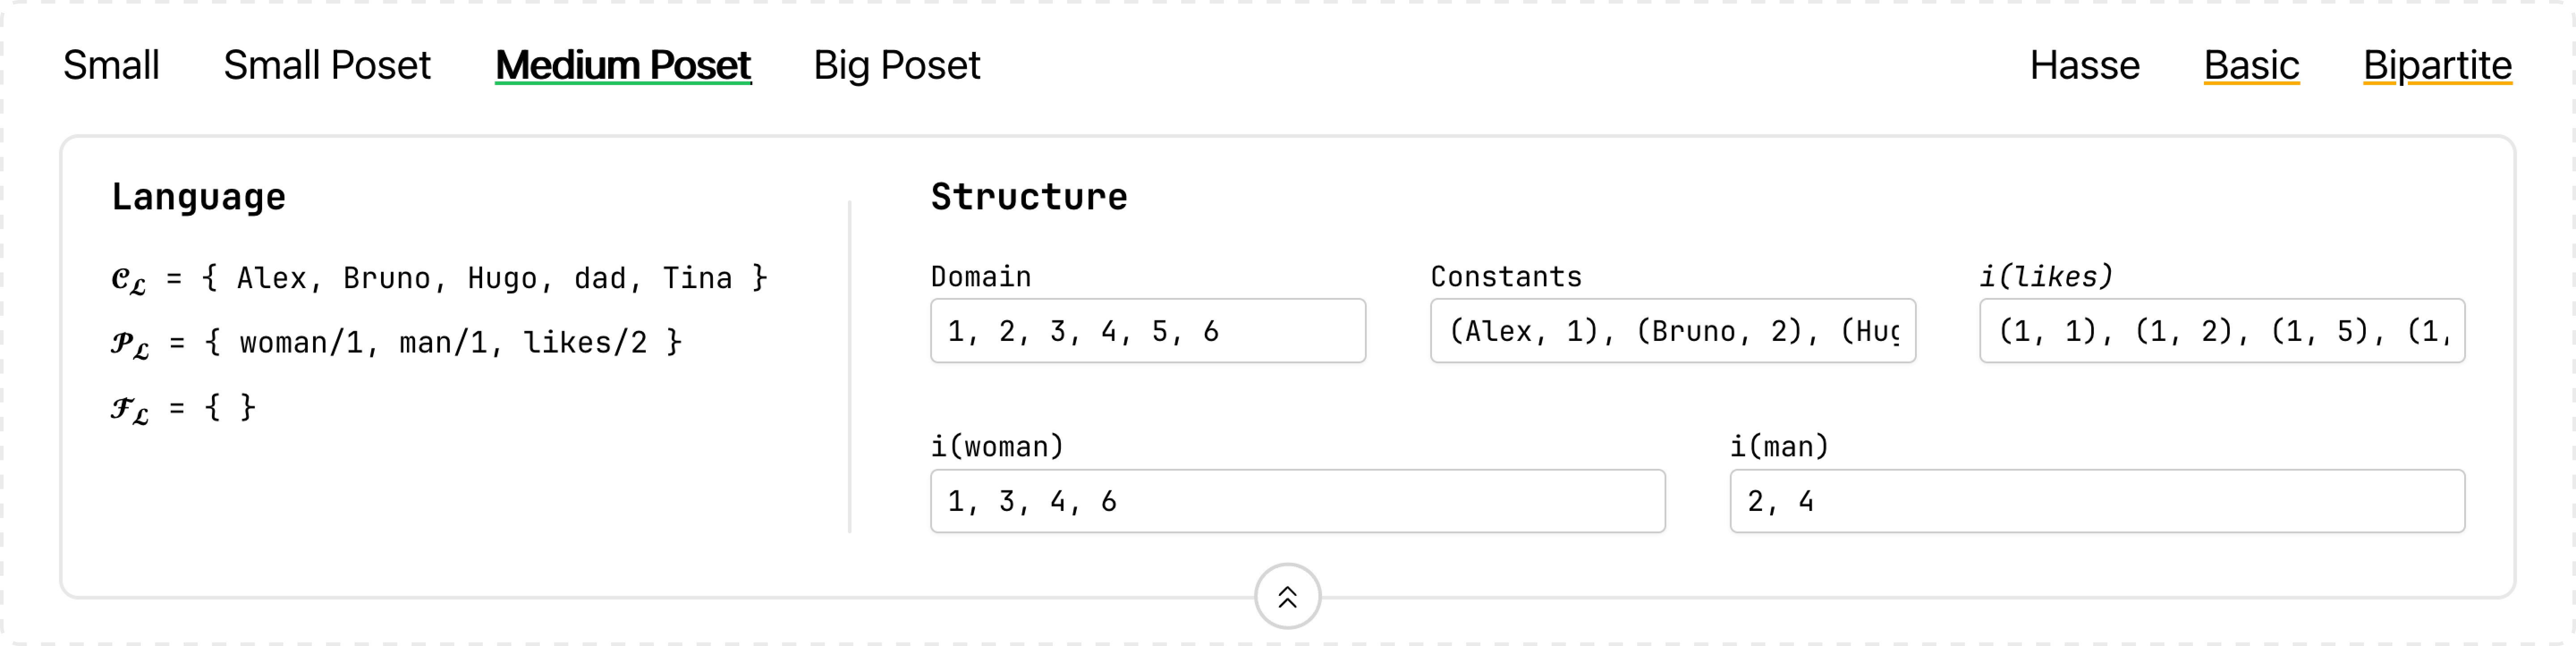
\includegraphics[width=1\textwidth]{images/demo_panel_2.png}}
    %popis obrazku
    \caption[Panel s jazykom a štruktúrou pilotnej implementácie.]{Panel s jazykom a štruktúrou pilotnej implementácie.}
    %id obrazku, pomocou ktoreho sa budeme na obrazok odvolavat
    \label{obr:demo_1}
\end{figure}

\begin{figure}
    \centerline{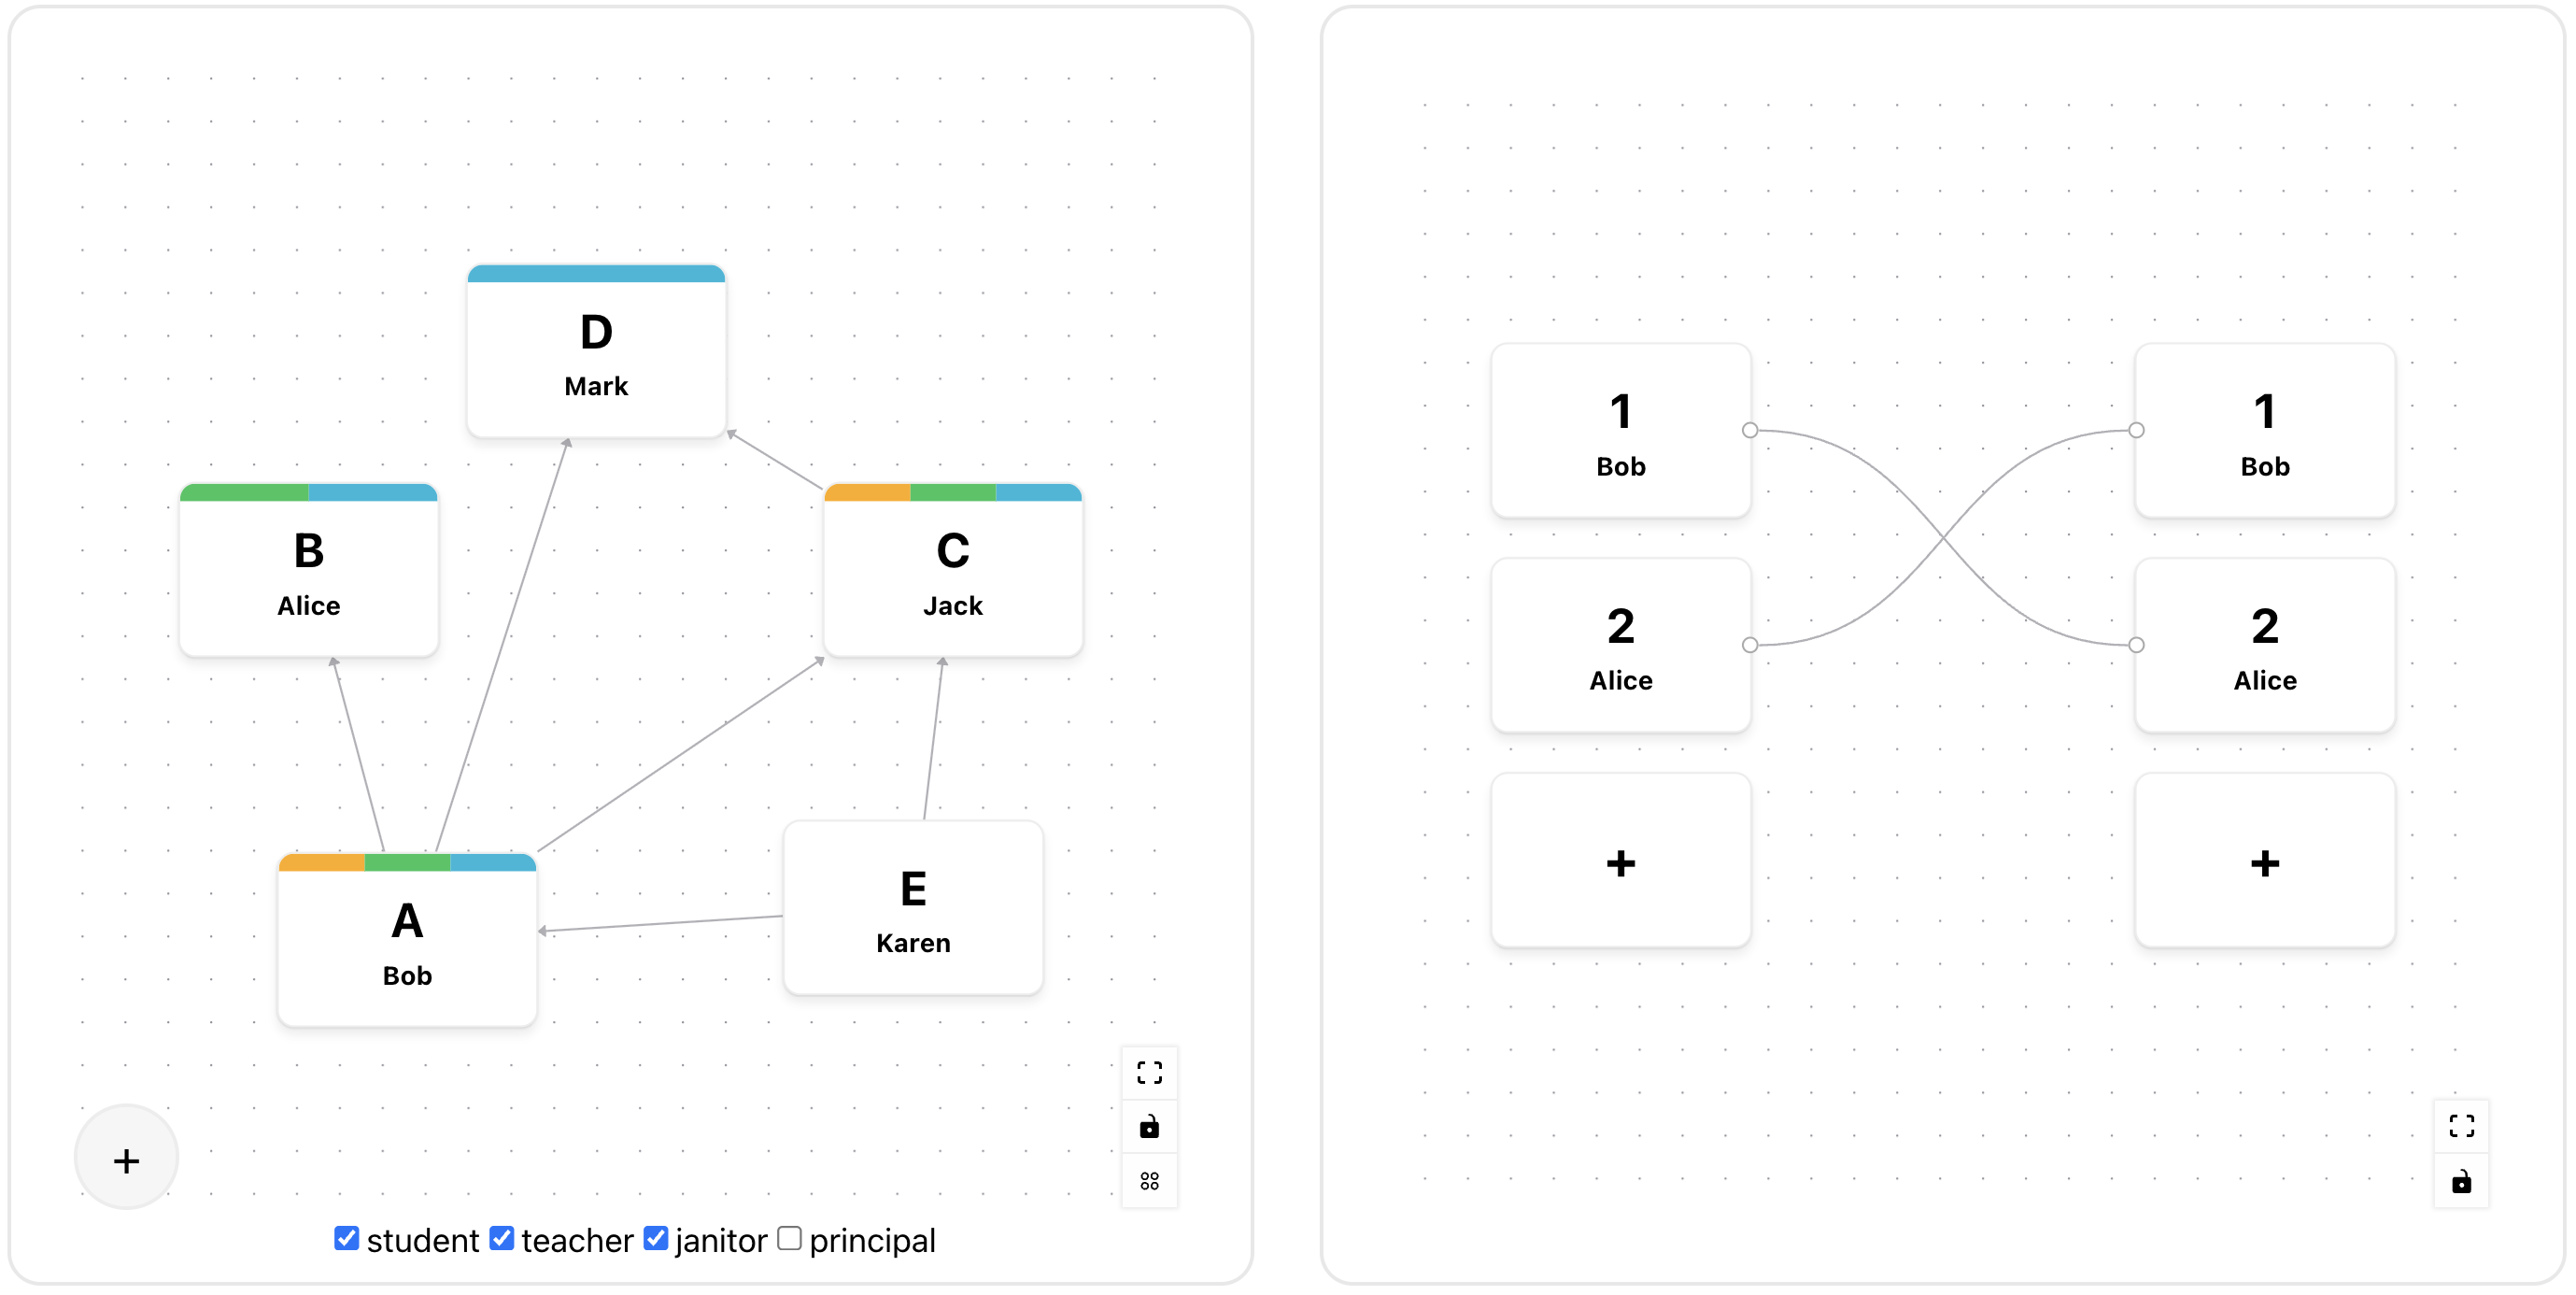
\includegraphics[width=1\textwidth]{images/demo_graph_1.png}}
    %popis obrazku
    \caption[Panel s orientovaným a bipartitným grafom pilotnej implementácie.]{Panel s orientovaným a bipartitným grafom pilotnej implementácie.}
    %id obrazku, pomocou ktoreho sa budeme na obrazok odvolavat
    \label{obr:demo_2}
\end{figure}

\begin{figure}
    \centerline{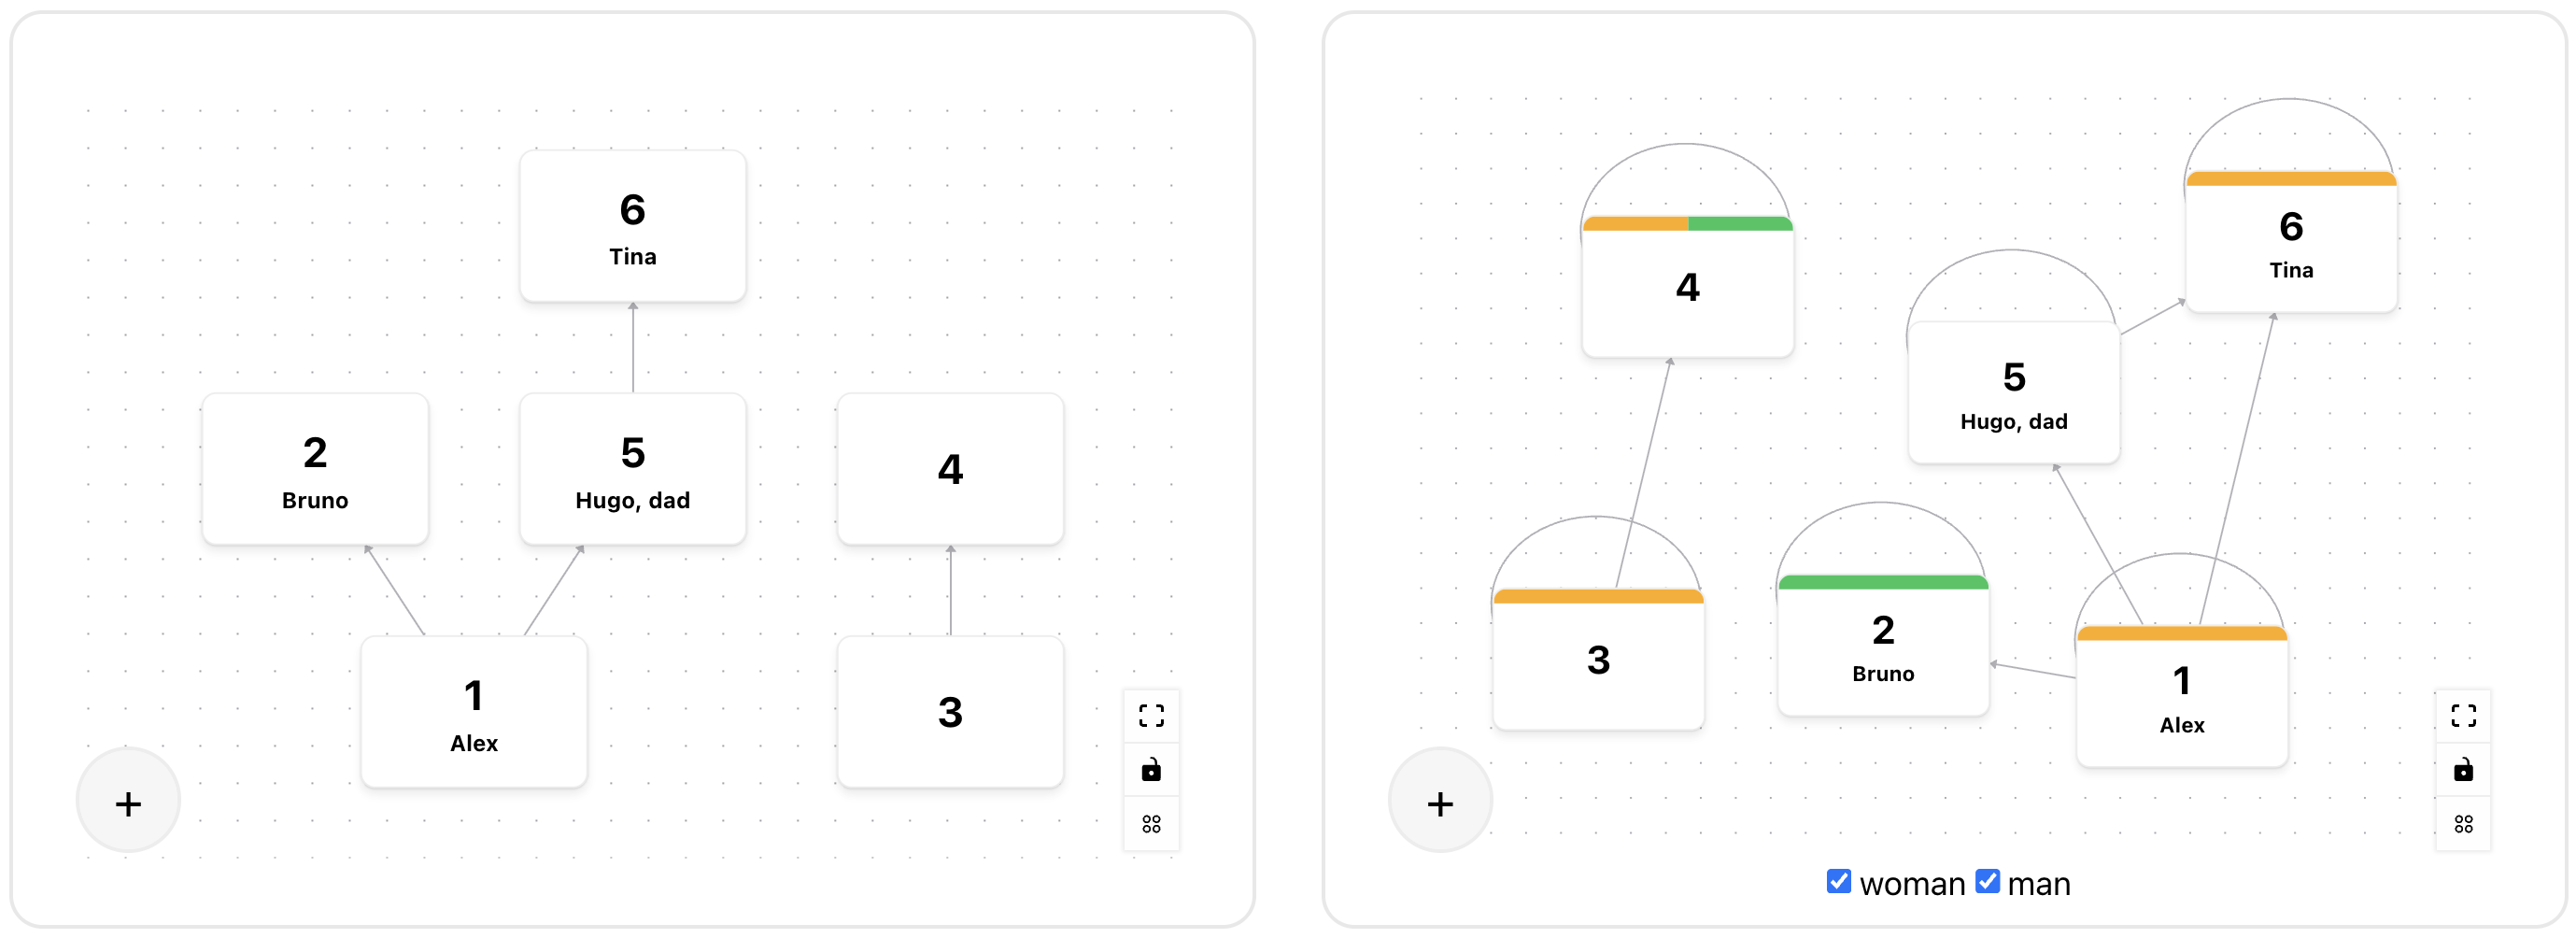
\includegraphics[width=1\textwidth]{images/demo_graph_2.png}}
    %popis obrazku
    \caption[Panel s Hasseho diagramom a orientovaným grafom pilotnej implementácie.]{Panel s Hasseho diagramom a orientovaným grafom pilotnej implementácie.}
    %id obrazku, pomocou ktoreho sa budeme na obrazok odvolavat
    \label{obr:demo_3}
\end{figure}

\section{Prínosy a získané poznatky}
\label{sec:pilot_rating}

Pilotná implementácia mi najmä pomohla získať lepšiu predstavu o tom, ako by jednotlivé grafy mali zdieľať spoločný stav a reagovať na jeho zmeny. Obzvlášť zaujímavé sa ukázalo byť prepojenie stavu Hasseho diagramu a orientovaného grafu, keďže Hasseho diagram, na rozdiel od ostatných dvoch reprezentácií, hrany redukuje. Tento problém je zatiaľ vyriešený na strane Hasseho diagramu vymazávaním nepotrebných hrán, to však môže byť pri väčších čiastočných usporiadaniach neefektívne, a teda bude potrebné tento prístup ešte prehodnotiť. Ďalej odhalila potrebu doladiť viaceré aspekty používateľského rozhrania ako intuitívnosť presúvania vrcholov, vytvárania hrán, mazania hrán alebo pridávania nových vrcholov. Tieto poznatky budú kľúčové pri tvorbe ďalších iterácií.